\documentclass[11pt,aspectratio=169]{beamer}
%%%%%%%%% GENERAL PACKAGES
%\usepackage[dvipsnames]{xcolor}
%\usepackage{pdfpages}
%\usetheme[progressbar=frametitle]{metropolis}
%\setbeamercolor{background canvas}{bg=white}
%\usepackage{appendixnumberbeamer}
%\usepackage{booktabs}
%\usepackage[scale=2]{ccicons}
%\usepackage{pgfplots}
%\usepgfplotslibrary{dateplot}
%\usepackage{xspace}
%\newcommand{\themename}{\textbf{\textsc{metropolis}}\xspace}
%\usepackage[absolute,overlay]{textpos}






%%%%%%%%% COLOR THEME

% Define some colors:
\definecolor{DarkFern}{HTML}{407428}
\definecolor{DarkCharcoal}{HTML}{4D4944}
\definecolor{AlertColor}{RGB}{89,124,158}
\definecolor{HighLight}{RGB}{96,95,134}
\definecolor{Important}{RGB}{234,122,133}
\definecolor{Yellow}{HTML}{00539C}
\colorlet{Fern}{DarkFern!85!white}
\colorlet{Charcoal}{DarkCharcoal!85!white}
\colorlet{LightCharcoal}{Charcoal!50!white}
\colorlet{HighLight2}{AlertColor}
\colorlet{DarkRed}{red!70!black}
\colorlet{DarkBlue}{blue!70!black}
\colorlet{DarkGreen}{green!70!black}
\definecolor{RoyalBlue}{HTML}{00539C}
\definecolor{Peach}{HTML}{EEA47F}
\definecolor{ForestGreen}{HTML}{2C5F2D}
\definecolor{MossGreen}{HTML}{E8FCC9}
\definecolor{SeaGreen}{HTML}{2E8B57}
% Use the colors:
\setbeamercolor{title}{fg=Fern}
\setbeamercolor{frametitle}{fg=MossGreen,bg=ForestGreen}
\setbeamercolor{normal text}{fg=Charcoal!70!black}
\setbeamercolor{block title}{fg=black,bg=Fern!25!white}
\setbeamercolor{block body}{fg=black,bg=Fern!10!white}
\setbeamercolor{block title alerted}{fg=black,bg=DarkRed!25!white}
\setbeamercolor{block body alerted}{fg=black,bg=DarkRed!10!white}
\setbeamercolor{alerted text}{fg=DarkRed}
\setbeamercolor{itemize item}{fg=Charcoal}



%%%%%%%%% OTHER COMMANDS
\newcommand{\indep}{\perp\!\!\! \perp}
\newcommand{\comment}[1]{}
\newcommand{\bs}{\boldsymbol}
\newcommand{\tr}{\text{trace}}
\newcommand{\sgn}{{\rm sgn}}
\def\T{\top}
%\newcommand{\det}{\text{det}}
\newcommand{\var}{\mathrm{var}}
\newcommand{\cC}{{\cal C}}
\renewcommand{\d}{{\rm d}}
\newcommand{\cG}{{\cal G}}
\newcommand{\cV}{{\cal V}}
\newcommand{\cE}{{\cal E}}
\newcommand{\cM}{{\cal M}}
\newcommand{\cP}{{\cal P}}
\newcommand{\cX}{{\cal X}}
\newcommand{\cY}{{\cal Y}}
\newcommand{\X}{\mathbf{X}}
\newcommand{\Y}{\mathbf{Y}}
\newcommand{\x}{\mathbf{x}}
\newcommand{\y}{\mathbf{y}}
\newcommand{\z}{\mathbf{z}}

\newcommand{\argmin}{\operatornamewithlimits{argmin}}
\newcommand{\eps}{\varepsilon}
\newcommand{\<}{\langle}
\renewcommand{\>}{\rangle}


%

\setbeamertemplate{navigation symbols}{}
\setbeamertemplate{footline}[text line]{%
    \hfill\strut{%
        \scriptsize\sf\color{black!60}%
        \quad\insertframenumber/\inserttotalframenumber
    }
    %\hfill
    }


\usenavigationsymbolstemplate{}
\setbeamersize{text margin left=.2cm,text margin right=.2cm} 
\addtobeamertemplate{frametitle}{}{\vspace{-1.2mm}}
\setbeamertemplate{itemize item}{$\bullet$}

\setbeamertemplate{itemize subitem}{\tiny\raise1.5pt\hbox{\donotcoloroutermaths$\blacktriangleright$}}
\setbeamertemplate{itemize subsubitem}{\tiny\raise1.5pt\hbox{\donotcoloroutermaths$\blacktriangleright$}}
\setbeamertemplate{enumerate item}{\insertenumlabel.}
\setbeamertemplate{enumerate subitem}{\insertenumlabel.\insertsubenumlabel}
\setbeamertemplate{enumerate subsubitem}{\insertenumlabel.\insertsubenumlabel.\insertsubsubenumlabel}
\setbeamertemplate{enumerate mini template}{\insertenumlabel}






\newcommand{\TODO}[1]{{\color{red}{[TODO: #1]}}}


\newcommand{\R}{\mathbb R}
\newcommand{\E}{\mathbb E}
\renewcommand{\P}{\mathbb P}


\DeclareMathOperator*{\cov}{cov}


\newsavebox{\zerobox}
\newenvironment{nospace}
{\par\edef\theprevdepth{\the\prevdepth}\nointerlineskip
  \setbox\zerobox=\vtop to 0pt\bgroup
  \hrule height0pt\kern\dimexpr\baselineskip-\topskip\relax
}
{\par\vss\egroup\ht\zerobox=0pt \wd\zerobox=0pt \dp\zerobox=0pt
  \box\zerobox}

\usepackage{soul}
\makeatletter
\let\HL\hl
\renewcommand\hl{%
  \let\set@color\beamerorig@set@color
  \let\reset@color\beamerorig@reset@color
  \HL}
  \makeatother



%\usecolortheme{whale}

\title[Calculus and Linear Algebra]{Lecture 5: Calculus and Linear Algebra}
\author[Piotr Zwiernik, Barcelona School of Economics]{Piotr Zwiernik \\ $\;$\\
Mathematics Brush-up\\ $\;$\\ $\;$\\

\includegraphics[width=1.5in]{img/bse.png}  
}
\date{}

%\beamerdefaultoverlayspecification{<+->}

\begin{document}
\begin{frame}
\titlepage
\end{frame}


%--------------- slide 2  ----------------%


%--------------- slide 1  ----------------%

\begin{frame}
\frametitle{Chapter 10: Differential equations}
\begin{small}
In many economic applications, we have to deal with time as a continuous variable, and to model those situations one uses \textcolor{blue}{differential equations}.
\vskip 12pt
\textcolor{blue}{Examples}: the most common models are exponential (savings account) or sub-exponential models (epidemic growth).
\vskip 12pt
\textcolor{blue}{Read}  sections 24.1 and 24.2 of Simon-Blume
\vskip 12pt
\textcolor{blue}{Exercises:} 24.5  (Simon-Blume)


\end{small}
\end{frame}

\begin{frame}
\frametitle{Ordinary differential equations}
\begin{small}
An \textcolor{blue}{ordinary first order differential equation} is an equation of the form $$\dot{y}(t)=F(y(t), t).$$
We usually write $$\dot{y}=F(y,t).$$
\vskip 12pt
 If $F$ only depends on $y$ it is called \textcolor{blue}{autonomous}: $\dot{y}=F(y)$.
\vskip 12pt
 \textcolor{blue}{Example 1: Exponential model} $\dot{y}=r y$ 
\vskip 10pt
 \textcolor{blue}{Solution :} $$y(t)=y(0) e^{rt}.$$

\begin{tiny}Proof: integrating: $\int_0^t \frac{dy}{y} =\int_0^t ds$, gives $\ln y(t)-\ln y(0)=rt$. Then take exponentials. \end{tiny}


\end{small}
\end{frame}

\begin{frame}
\frametitle{Ordinary differential equations}
\begin{small}
\textcolor{blue}{Example 2: Exponential model} $\dot{y}=r(t) y$ 
\vskip 10pt
 \textcolor{blue}{Solution :} $$y(t)=y(0) e^{\int_0^t r(s) ds}.$$

\begin{tiny}Proof: integrating: $\int_0^t \frac{dy}{y} =\int_0^t r(s) ds$, gives $\ln y(t)-\ln y(0)=\int_0^t r(s) ds$. Then take exponentials. \end{tiny}
\vskip 12pt
\textcolor{blue}{Example 3: Exponential model} $\dot{y}=r(t) y+b(t)$, 
\vskip 12pt
\textcolor{blue}{Solution :} $y(t)=\left(y(0) +\int_{0}^t b(s) e^{-\int_0^s r(u) du}ds \right)e^{\int_0^t r(s) ds} .$
\vskip 12pt
\begin{tiny}Proof: write $(\dot{y}-r(t) y=b(t))e^{-\int_0^t r(s) ds} $,
and integrate $\int_0^t \frac{d}{ds}\left(y(s)e^{-\int_0^s r(u) du} \right)  =\int_0^t b(s)e^{-\int_0^s r(u) du}ds$.  \end{tiny}


\end{small}
\end{frame}


\begin{frame}
\frametitle{Ordinary differential equations}
\begin{small}
\textcolor{blue}{Example 4: Sub-Exponential model} $\dot{y}=r y^p,$
$p \in (0,1)$. 
\vskip 10pt
 \textcolor{blue}{Solution :} $$y(t)=(y(0)^{1-p} +(1-p) rt)^{1/(1-p)}.$$

\begin{tiny}Proof: integrating: $\int_0^t \frac{dy}{y^p} =rt$, gives $y(t)^{1-p}=y(0)^{1-p}+(1-p)rt$. \end{tiny}


\begin{figure}
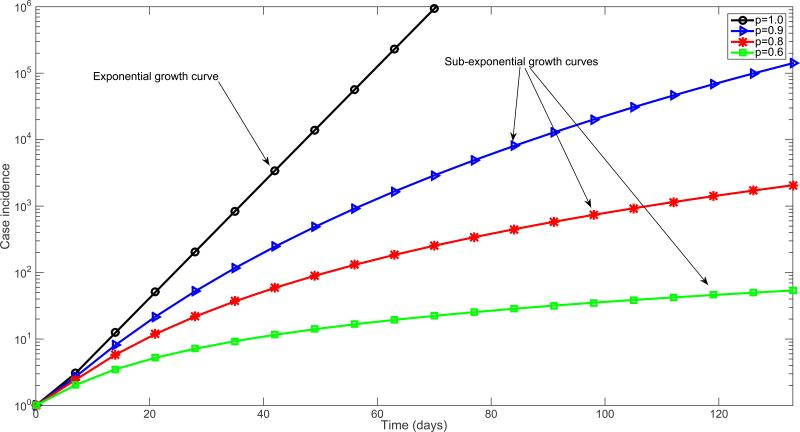
\includegraphics[width=3in]{img/growth} 
\end{figure}
\end{small}
\end{frame}

\begin{frame}
\frametitle{Example 5: Logistic growth model}
\begin{small}
$$\dot{y}=y(1-y), \quad \begin{tiny}0<y(0) <1, \quad 1=\text{carrying capacity}\end{tiny}$$
\vskip 12pt
\textcolor{blue}{Solution:} $
y(t)=\frac{1}{1+a e^{-t}}, \quad a=\frac{1}{y(0)}-1$
\end{small}
\begin{tiny}
Proof: Use that $\frac{1}{y(1-y)}=\frac{1}{y}+\frac{1}{1-y}$ and integrate
\end{tiny}
\begin{figure}
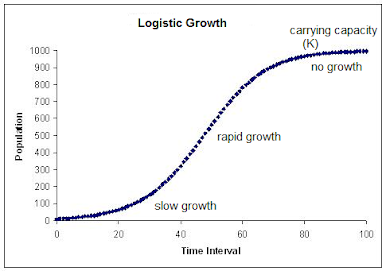
\includegraphics[width=2.5in]{img/LG.png} 
\end{figure}
\end{frame}

\begin{frame}
\frametitle{
 Cobb-Douglas production function}
\begin{small}
The solution to $
\frac{\partial P}{\partial L}=\alpha \frac{P}{L}
$ with $K=K_0$ is
$$P(L, K_0)=C_1(K_0) L^{\alpha}.$$
\begin{tiny}Integrate $\int \frac{dP}{P}=\alpha \int \frac{dL}{L}$
so $\ln(P)=\alpha \ln(cL)$ \end{tiny}
\vskip 12pt
The solution to
$
\frac{\partial P}{\partial K}=\beta \frac{P}{K}
$
with $L=L_0$ is $$P(L_0, K)=C_2(L_0) K^{\beta}.$$
\vskip 10pt
 Combining both equations we get  $$P(L, K)=b L^{\alpha} K^{\beta},$$ where  $b$ is a constant.

\vskip 12pt
 Assumption 1 shows that  $\alpha, \beta>0$.


\end{small}
\end{frame}




\begin{frame}
\frametitle{ Second  order differential equation: an example}
\begin{small}
 Let $x \rightarrow u(x)$ the \textcolor{blue}{utility function} for  wealth $x$. 
\vskip 10pt
The Relative Risk-Aversion is $-\frac{x u''(x)}{u'(x)}$

\vskip 10pt

Assuming that the  \textcolor{blue}{relative risk aversion is 1}, we obtain the second order differential equation
$$
u''(x)=-\frac{u'(x)}{x}.
$$


Let $v(x)=u'(x)$.  Then, the equation becomes a first order differential equation
$$
\frac{dv}{dx}=-\frac{v}{x}.
$$

\vskip 10pt
The \textcolor{blue}{solution} is  $v(x)=k_1 x^{-1}$. Therefore $u(x)=k_2+k_1 \ln  x$.

\begin{tiny}
Integrate $\int \frac{dv}{v}=-\int \frac{dx}{x}$.
\end{tiny}


\end{small}
\end{frame}


\end{document}
